\documentclass{beamer}
% 
% Choose how your presentation looks.
% 
% For more themes, color themes and font themes, see:
% http://deic.uab.es/~iblanes/beamer_gallery/index_by_theme.html
% 
\mode<presentation>
{
  \usetheme{Berlin}      % or try Darmstadt, Madrid, Warsaw, ...
  \usecolortheme{default} % or try albatross, beaver, crane, ...
  \usefonttheme{default}  % or try serif, structurebold, ...
  \setbeamertemplate{navigation symbols}{}
  \setbeamertemplate{caption}[numbered]
} 

\usepackage{default}
%\usepackage[english]{babel}
%\usepackage[T1]{fontenc}
%\usepackage[utf8]{inputenc}
\usepackage{natbib}
\usepackage{graphicx}
%\usepackage{subfig}

\graphicspath{{figures/}}
\bibliographystyle{alpha}
\renewcommand\bibfont{\scriptsize}

%\captionsetup{compatibility=false}

\title{Selecting Representative Models from Time Series Ensembles}
\author{Guilherme Gon\c{c}alves Schardong}
\date{\today}

\begin{document}
	
\begin{frame}
  \titlepage
\end{frame}

\begin{frame}{Outline}
  \tableofcontents
\end{frame}

\section{Introduction}
\begin{frame}
  \tableofcontents[currentsection]
\end{frame}

\begin{frame}{Introduction}
  \begin{itemize}
    \item Increased use of ensemble based methods;
    \item Difficulty to ``sift'' through this data and discover useful knowledge;
    \item Need of approaches to make the amount of data more tractable;
  \end{itemize}
\end{frame}

\begin{frame}{Example of an Ensemble}
  \begin{figure}
    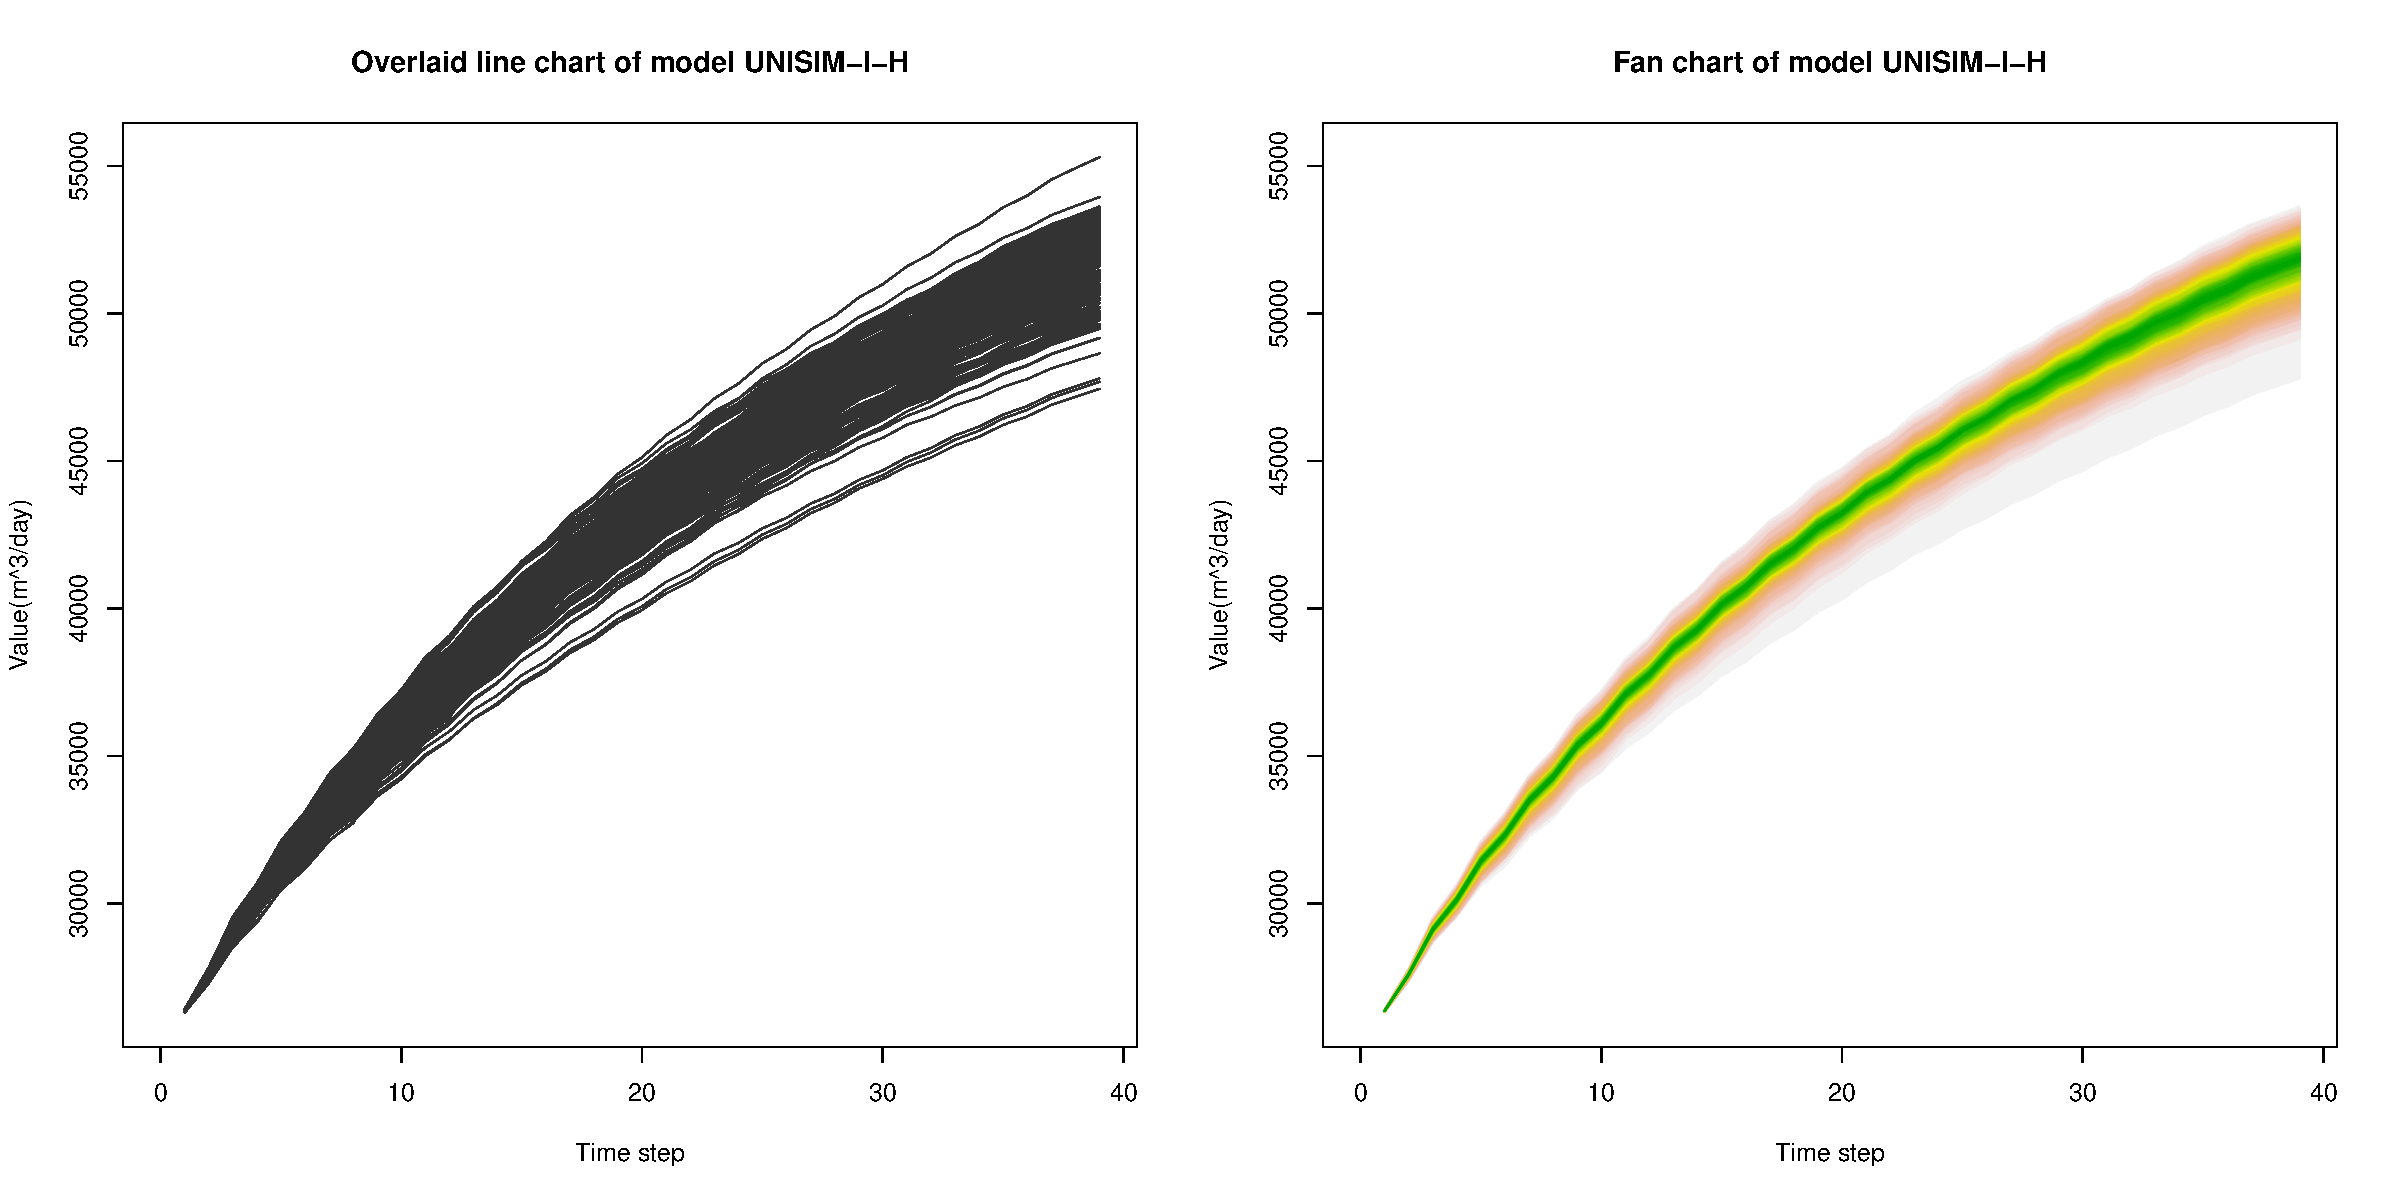
\includegraphics[width=\columnwidth]{line-fan.pdf}
    \caption{Example of a time series ensemble.}
    \label{fig:sample}
  \end{figure}
\end{frame}

\section{Research Question}
\begin{frame}
  \tableofcontents[currentsection]
\end{frame}

\begin{frame}{Research Question}
  \begin{itemize}
    \item Given a large set of models, how can a statistically significant subset be selected, such that analysis tasks done with the subset are equivalent to using the original set?
  \end{itemize}
\end{frame}

\section{Systematic Mapping}
\begin{frame}
  \tableofcontents[currentsection]
\end{frame}

\subsection{Planning}
\begin{frame}{Reference Databases}
  \begin{itemize}
  \item ACM;
  \item SpringerLink;
  \item ScienceDirect;
  \item IEEExplore;
  \item Scopus.
  \end{itemize}
\end{frame}

\begin{frame}
  Possible Queries:
  \begin{itemize}
    \item (Statistical OR Representative) AND ``Model Selection'' AND (Ensemble OR Uncertainty OR Clustering OR Optimization OR MinMax);
  \end{itemize}
\end{frame}

\subsection{Preliminary Results}
\begin{frame}{Papers per source}
  \begin{table}[]
    \centering
    \caption{Papers Per Source}
    \label{my-label}
    \begin{tabular}{lllllll}
      & \textbf{ACM} & \textbf{\begin{tabular}[c]{@{}l@{}}Springer\\ Link\end{tabular}} & \textbf{\begin{tabular}[c]{@{}l@{}}Science\\ Direct\end{tabular}} & \textbf{IEEExplore} & \textbf{Scopus} & \textbf{Total} \\ \hline
      Total & 11           & 10                                                               & 8                                                                 & 32                  & 84              & 145            \\
      E.C.  & 4            & 3                                                                & 4                                                                 & 7                   & W.I.P.             & \textgreater18
    \end{tabular}
  \end{table}
\end{frame}

\begin{frame}
  \begin{figure}
    \centering
    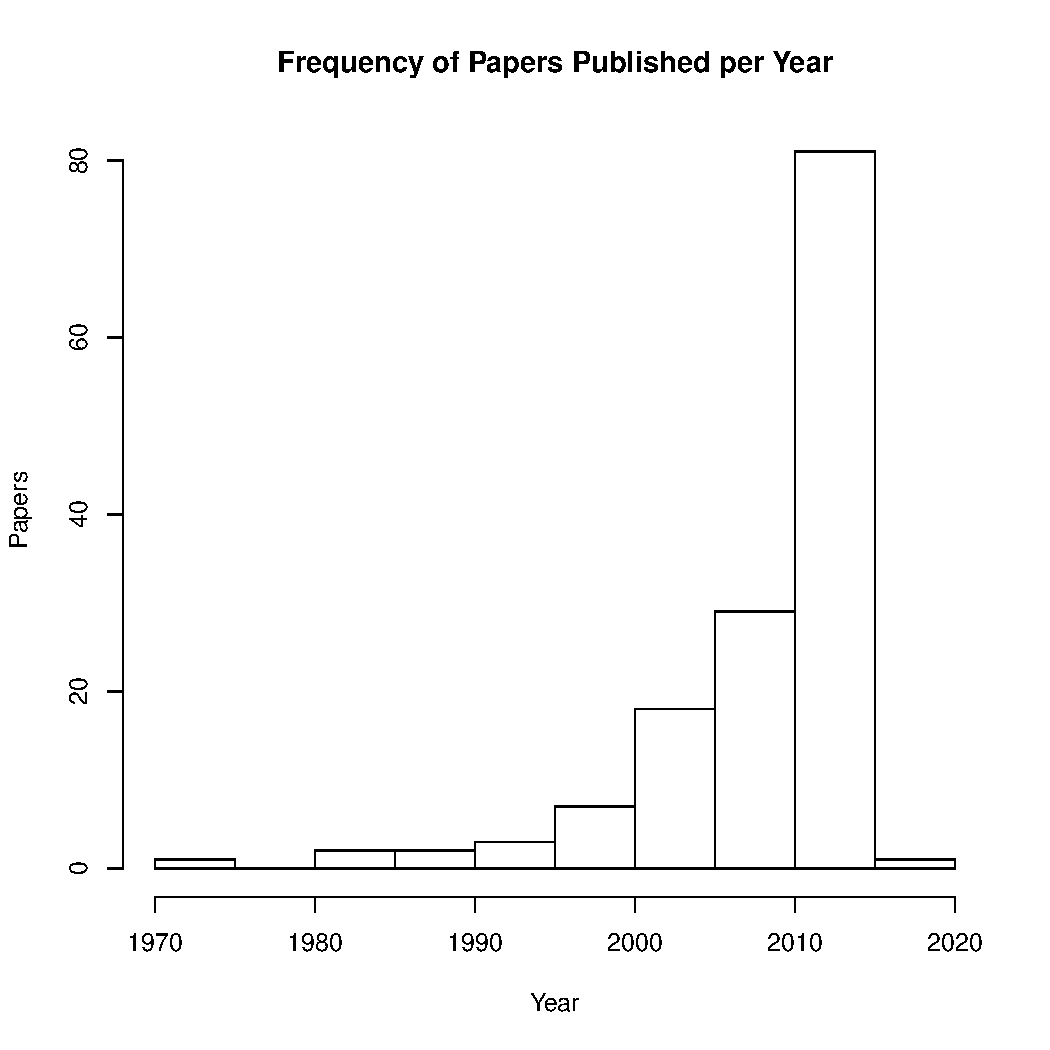
\includegraphics[width=0.7\columnwidth]{hist-paper-year.pdf}
    \label{fig:hist-paper-year}
  \end{figure}
\end{frame}

\subsection{Preliminary Conclusions}
\begin{frame}{Systematic Mapping Preliminary Conclusions}
  \begin{itemize}
  \item Several papers related to classification tasks;
  \item Similar results in clustering approaches (Ensemble of clusterings and consensus clustering);
  \item No time series ensemble selection techniques;
    \begin{itemize}
    \item Contribution potential.
    \end{itemize}
  \end{itemize}
\end{frame}

\section{}
\begin{frame}
  \titlepage
\end{frame}

\end{document}
